{
\section{Definition of the Brownian web}
\label{sec:brownian-web-definition}

The Brownian web is the continuum scaling limit of a system of
independent coalescing random walks (see []).  Constructing the
continuum version raises several technical difficulties addressed in
[] [] [] . One way to deal with the difficulties is to introduce the
structure of flows as detailed in [].  Nonetheless all the
constructions share the following property, which we use as a
definition, at the expense of uniqueness:

  Denote $\simplex=\{(s, t) \in \R^2 : s \le t\}$.
  A Brownian web on a probability space $\Omega$ is a (jointly)
  measurable mapping $\webnoargs : \Omega \cross \simplex \cross \R
  \to \R$, $(\omega, (s, t), x) \mapsto \web{s}{t}{x}$ (supressing
  $\omega$ in the notation) such that for every finite collection of
  starting points $(s_1, x_1),(s_2, x_2),...,(s_n, x_n)$, the
  collection of processes $\web{s_1} {\cdot}{x_1},
  \web{s_2}{\cdot}{x_2},...,\web{s_n}{\cdot}{x_n}$
  forms a system of $n$ independent-coalescing Brownian motions.

  A system of $n$ independent-coalescing Brownian motions is a finite
  collection of stochastic processes $(X_1, X_2,...,X_n)$ such that
  each $X_i$ starts at some point $x_i$ at some time $s_i$, and $(X_1,
  X_2,...,X_n)$ are independent until the first time $T$ at which
  $X_i(T)=X_j(T)$ for some $i\neq j$. From this time onwards $X_i(T)$
  and $X_j(T)$ coalesce and continue with the rest of the $X_k$ (for
  $k\neq i,j$) as a system of $n-1$ independent-coalescing Brownian motions.
  Several trajectories of a Brownian web can be seen in Figure
  \ref{fig:bw-trajectories}.

  \newcommand{\F}{\mathcal{F}}
We conclude this section by indroducing a notation for independent
factorization of $\sigma$-fields.
  For $\sigma$-fields $\F_a$, $\F_b$, $\F_c$ we write $\F_a = \F_b
  \tensor \F_c$ when $\F_b$ and $\F_c$ are independent, and $\F_a$
  is generated by $\F_b$ and $\F_c$ (up to sets of measure $0$).

\begin{figure}
   \centering
   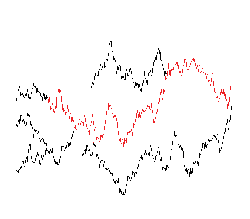
\includegraphics[scale=2]{sometraj.eps}
   \caption{Some trajectories of the Brownian web. A particular trajectory is marked.}
  \label{fig:bw-trajectories}
\end{figure}
}
